%% =========================================================================
%% Course Report Template (XeLaTex)
%% 
%% Author: 赵苡积 (云南大学信息学院)
%% GitHub: https://github.com/yijizhao
%% 
%% =========================================================================
\documentclass{style/course-report}

\usepackage{subfigure}
\hypersetup{
    colorlinks=true,
    linkcolor=blue,
    filecolor=black,
    urlcolor=black,
    citecolor=blue,
}


% ================= 填写封面信息 =================
\coursetitle{《深度学习》实训作业} %课程报告标题
\expname{前馈神经网络实验} %题目
\studentname{张三} %姓名
\studentid{20230212} %学号
\major{计算机科学与技术} %专业
\expdate{\today} %日期，默认当天，也可以根据自己需求修改

\begin{document}

% 生成封面
\makecover


\section{实训内容}

1、	理解人工神经元的结构与工作原理：掌握 Sigmoid、Tanh、ReLU 等常见激活函数的定义、实现及选择依据。

2、	掌握前馈神经网络的组成结构（输入层、隐藏层、输出层）与参数学习流程（前向传播、损失计算、反向传播、参数更新）。

3、	能够分别通过手动实现（基于 Tensor）和调用 Torch.nn 组件实现前馈神经网络，解决多分类任务（如手写数字识别）。

4、	完成激活函数对比实验与网络结构超参数（隐藏层层数、隐藏单元数）影响分析实验，能从训练时间、准确率、损失变化等角度分析实验结果。



\subsection{基于基础算子搭建前馈神经网络}
（1）任务：基于Pytorch、TensorFlow等深度学习框架中的基础算子，手动实现一个前馈神经网络识别手写体图像中的数字。

（2）目的：掌握实现手动编写前馈神经网络的方法。

（3）要求：从训练时间、预测精度、Loss变化等角度分析实验结果。

\subsection{基于神经网络组件库搭建前馈神经网络}
（1）任务：基于Pytorch、TensorFlow等深度学习框架中的神经网络组件库，实现一个前馈神经网络识别手写体图像中的数字。

（2）目的：掌握基于神经网络组件库实现前馈神经网络的方法。

（3）要求：从训练时间、预测精度、Loss变化等角度分析实验结果。

\subsection{激活函数对比分析}
（1）任务：xx。
（2）目的：xx。
（3）要求：xx。

\subsection{网络结构参数影响分析}
（1）任务：xx。
（2）目的：xx。
（3）要求：xx。

\section{方案设计}
% 本部分需包含关键核心代码（非整个工程代码）。为了代码片段尽量的美观、统一，建议附代码片段时只附加关键的片段。


\subsection{基于基础算子搭建前馈神经网络}
% 方案介绍：描述、形式化、示意图/流程图、核心代码（含关键注释）等。

代码样例：

\begin{lstlisting}[language=Python]
# ================= 冒泡排序算法实现 =================
def bubble_sort(arr):
    n = len(arr)
    # 遍历所有数组元素
    for i in range(n):
        # Last i elements are already in place
        for j in range(0, n-i-1):
            # 如果当前元素大于下一个元素，则交换它们
            if arr[j] > arr[j+1]:
                arr[j], arr[j+1] = arr[j+1], arr[j]
    return arr

# 测试代码
if __name__ == "__main__":
    my_list = [64, 34, 25, 12, 22, 11, 90]
    sorted_list = bubble_sort(my_list)
    print("排序后的数组:", sorted_list)
\end{lstlisting}

\subsection{基于神经网络组件库搭建前馈神经网络}
% 方案介绍：描述、形式化、示意图/流程图、核心代码（含关键注释）等。

\subsection{激活函数对比分析}
% 方案介绍：描述、形式化、示意图/流程图、核心代码（含关键注释）等。

\subsection{网络结构参数影响分析}
% 方案介绍：描述、形式化、示意图/流程图、核心代码（含关键注释）等。



\section{实验设置}

\subsection{数据集}
% 如果有数据集（公开数据集/合成数据），需要介绍数据集的相关信息，包括但不限于：数据的来源（有文献源应引用）、数据的基本统计信息、部分数据的可视化、数据的清洗操作、数据标准化、数据增强手段等。

例如，本次实训基于MNIST手写体数据集\cite{lecun2002gradient}，其包含60,000个用于训练的图像样本和10,000个用于测试的图像样本，每张图像为固定大小（28$\times$28像素），像素值为0或1。


\subsection{实验环境}
% 介绍软硬件环境信息等，包括但不限于服务器环境、CUDA版本、语言等信息。


\subsection{模型配置细节}
% 介绍模型超参数的设置范围以及如何选定的超参数，如模型的隐维度、层数、优化器、学习率、总训练轮数、早停轮数、正则系数、dropout率等超参数说明，具体说明如层数$l\in\{1,2,\dots,5\}$，通过网格搜索，并在验证集上设置早停确定最佳超参为xxx。

\subsection{评价指标}
% 简介用什么样的指标来评判你的实验结果，比如准确率等指标的简介、定义（含形式化）

\begin{equation}
    \mathrm{ACC} = \frac{A}{B}
    \label{eq:acc}
\end{equation}


\section{实验结果与分析}
% 实验结果包括程序运行结果以及对结果的分析，合理利用折线图、柱状图、表格等多样化的手段丰富实验结果，并且结合结果进行适当的分析。

\subsection{基于基础算子搭建前馈神经网络}

示例表格样式如下：
\begin{table}[H]
    \centering
    \caption{实验结果数据表} % 每个表格应有编号和标题，编号和标题应写在表格上方正中
    \begin{tabular}{ccc}
        \toprule
        参数 & 准确率 / \% & 训练时间 / s \\ % 表格中量与单位之间用“/”分隔
        \midrule
        设置 A & 92.5 & 120 \\
        设置 B & 95.1 & 180 \\
        \bottomrule
    \end{tabular}
    \label{tab:example}
\end{table} % 表格应为三线表

推荐使用python中的matplotlib绘图，加入自动裁剪命令，存为pdf，dpi设为300，注意图中文字应尽量使用中文。单图示例样式如下：
\begin{figure}[H]
    \centering
    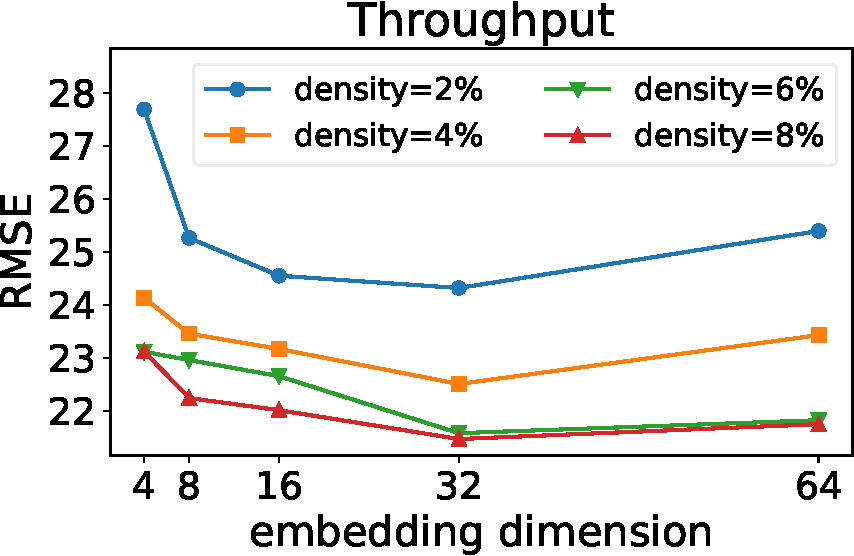
\includegraphics[width=0.70\textwidth]{figs/example.pdf}
    \caption{xxx曲线}
    \label{fig:example}
\end{figure}

多图并列示例图表样式如下：
%%%%%%%%%%%%%%%%%%%%%%%%%%%%%%%%%%%%%%%%%%%%
%                 Figure                  %
%%%%%%%%%%%%%%%%%%%%%%%%%%%%%%%%%%%%%%%%%%%%
\begin{figure}[ht]
    \centering
    \subfigure[XXX1曲线]{
        \label{fig:example_a}
        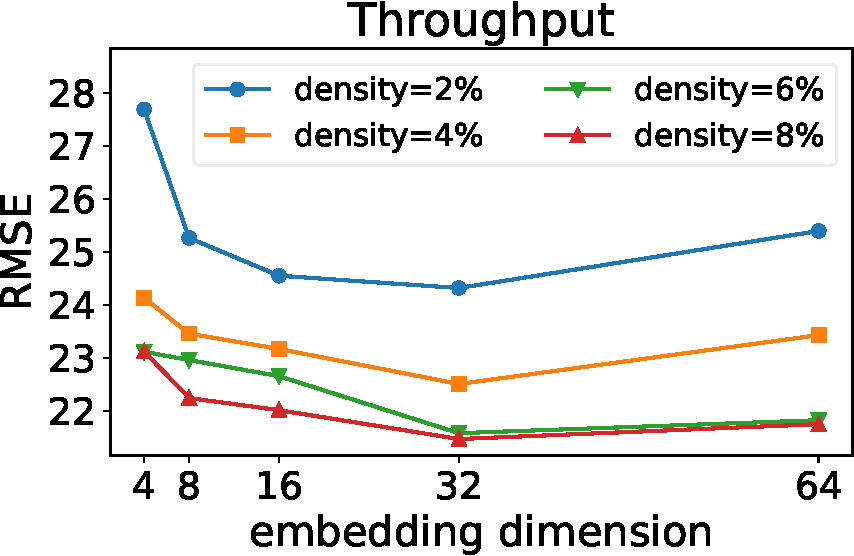
\includegraphics[width=0.45\linewidth]{figs/example.pdf}
    }\hfill
    \subfigure[XXX2曲线]{
        \label{fig:example_b}
        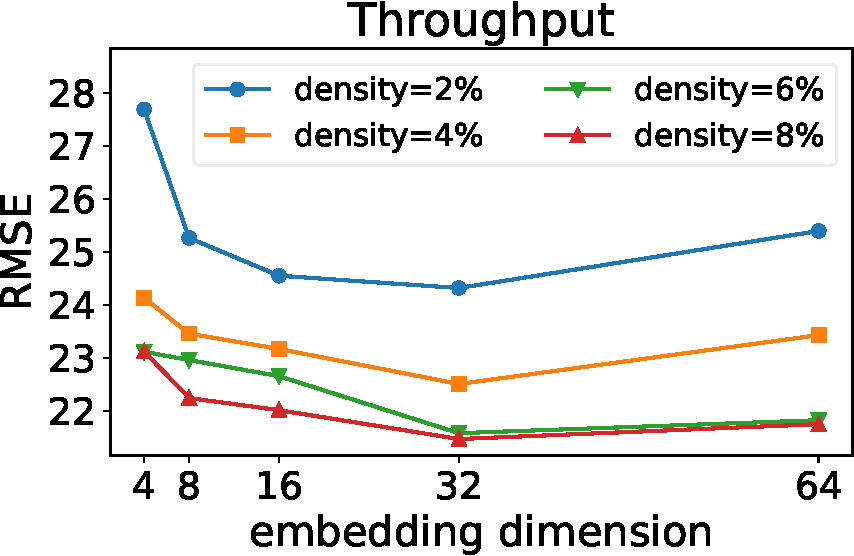
\includegraphics[width=0.45\linewidth]{figs/example.pdf}
    }\hfill
    \subfigure[XXX3曲线]{
        \label{fig:example_c}
        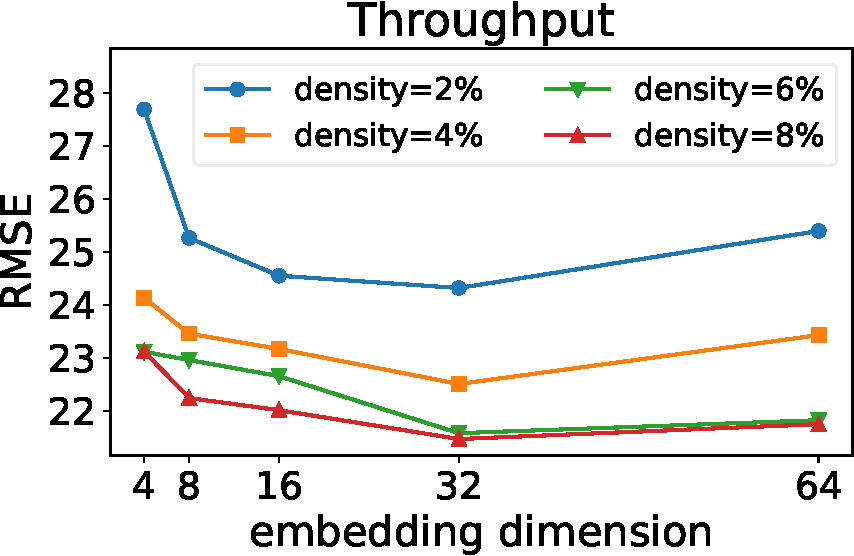
\includegraphics[width=0.45\linewidth]{figs/example.pdf}
    }\hfill
    \subfigure[XXX4曲线]{
        \label{fig:example_d}
        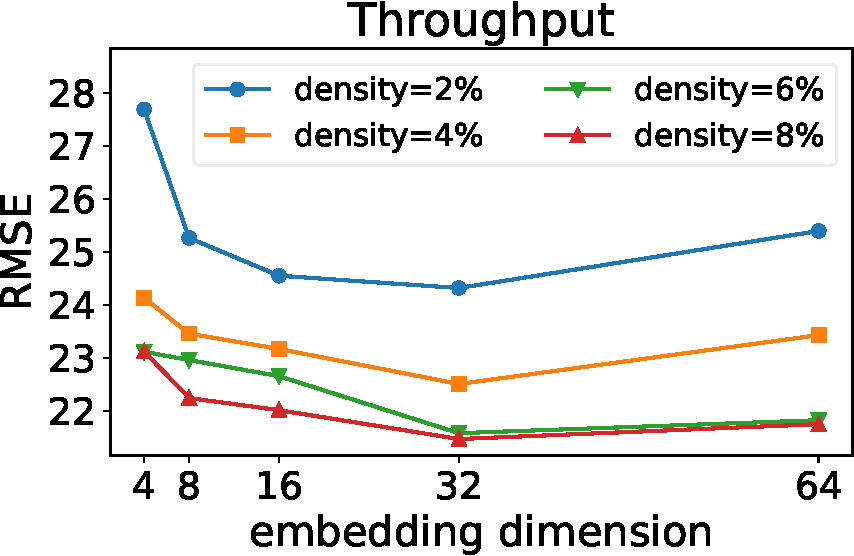
\includegraphics[width=0.45\linewidth]{figs/example.pdf}
    }
    \caption {\label{fig:multi1}嵌入维度的影响.}
\end{figure}

图、表、公式、算式等，一律用阿拉伯数字分别依序连续编排序号，其标注形式应便于互相区别，可分别为：图\ref{fig:example}、图\ref{fig:example_a}、表\ref{tab:example}、公式\ref{eq:acc}等。

\subsection{基于神经网络组件库搭建前馈神经网络}

\subsection{激活函数对比分析实验}

\subsection{网络结构参数影响分析实验}

\section{心得体会}
% 本部分主要包含自己做实验过程中遇到的困难以及解决办法，通过做实验自己有哪些收获和体会，以及不足等等。


 
\bibliography{ref}
% 参考文献主要包含实验过程中涉及到的参考资料或者借鉴别人的材料等，如无可删除本节。 



\end{document}